\documentclass{article}
\usepackage[utf8]{inputenc}
%\usepackage[default]{sourcecodepro}
\usepackage[T1]{fontenc}
\usepackage{amsmath}
\usepackage{amssymb}
\usepackage{enumitem}
\usepackage{geometry}
%\usepackage{fancyhdr}
\usepackage{color,xcolor,colortbl}
\usepackage{longtable}
\usepackage{graphicx}
\usepackage{multirow}
\usepackage{layout}
\usepackage{vwcol} 
\usepackage{changepage}
\usepackage{multicol}
\usepackage{nopageno}
\usepackage{fontawesome}
\usepackage{setspace}
%\usepackage{lmodern}
 %\fontfamily{cmss}\selectfont
\usepackage[compact]{titlesec}
\titlespacing{\section}{0pt}{0pt}{0pt}
%\usepackage[hyphens]{url}
\usepackage[breaklinks]{hyperref}
\newcommand*\ruleline[1]{\par\noindent\raisebox{.8ex}{\makebox[\linewidth]{\hrulefill\hspace{1ex}\raisebox{-.8ex}{#1}\hspace{1ex}\hrulefill}}}
\definecolor{Gray}{gray}{0.55}
\definecolor{darkgray}{gray}{0.35}
\definecolor{blue}{rgb}{0.01,0.28,1}
\definecolor{cyan}{rgb}{0,0.7,0.7}
\definecolor{chamoisee}{rgb}{0.63, 0.47, 0.35}
\definecolor{darklava}{rgb}{0.28, 0.24, 0.2}
\definecolor{armygreen}{rgb}{0.29, 0.33, 0.13}
\definecolor{darkbrown}{rgb}{0.4, 0.26, 0.13}
\definecolor{bulgarianrose}{rgb}{0.28, 0.02, 0.03}
\definecolor{beaver}{rgb}{0.62, 0.51, 0.44}
\definecolor{lighttaupe}{rgb}{0.7, 0.55, 0.43}
\definecolor{otterbrown}{rgb}{0.4, 0.26, 0.13}
\definecolor{mediumtaupe}{rgb}{0.44, 0.38, 0.3}
\definecolor{palebrown}{rgb}{0.6, 0.46, 0.33}
\definecolor{purpletaupe}{rgb}{0.31, 0.25, 0.3}
\definecolor{pastelbrown}{rgb}{0.51, 0.41, 0.33}
\definecolor{tealgreen}{rgb}{0.0, 0.51, 0.5}
\definecolor{toolbox}{rgb}{0.45, 0.42, 0.75}
\definecolor{cinereous}{rgb}{0.6, 0.51, 0.48}
\definecolor{warmblack}{rgb}{0.0, 0.26, 0.26}
\definecolor{cadmiumgreen}{rgb}{0.0, 0.42, 0.24}
\definecolor{green}{rgb}{0.46, 1, 0.44}
\definecolor{roseebony}{rgb}{0.4, 0.3, 0.28}
\definecolor{darkblue}{rgb}{0, 0, 0.3}
\definecolor{paletaupe}{rgb}{0.74, 0.6, 0.49}
\definecolor{rawumber}{rgb}{0.51, 0.4, 0.27}
\definecolor{darktan}{rgb}{0.57, 0.51, 0.32}
\definecolor{sepia}{rgb}{0.44, 0.26, 0.08}
\definecolor{umber}{rgb}{0.39, 0.33, 0.32}
\definecolor{indianred}{rgb}{0.6, 0.26, 0.26}
\definecolor{WHITE}{gray}{1}
\hypersetup{
colorlinks = true,
linkcolor = blue,
urlcolor = green
}
\geometry{
 a4paper,
 right=10mm,
 left=10mm,
 top=8mm,
 bottom=10mm,
 nohead
 }
\setlength{\arrayrulewidth}{0.1mm}
\setlength{\tabcolsep}{10pt}
\renewcommand{\arraystretch}{1}
\urlstyle{same}

%\pagestyle{fancy}
%\fancyhf{}
%\renewcommand{\headrulewidth}{0pt}


%\newcolumntype{a}{>{\columncolor{armygreen}}p}

\begin{document}
\flushleft{


%\hline
%\multicolumn{5}{|c|} \\
%\hline
\parbox[][32mm][t]{19cm}{{\fbox{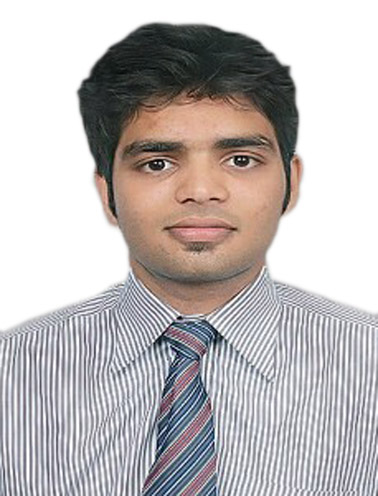
\includegraphics[width=2.5cm, height=3cm]{Photo.jpg}}} \hfill \parbox[][40mm][t]{16cm}{\flushright{
{\huge {\uppercase{\textbf{Prahlad}}}}\\ \vspace{5mm}{\huge {\uppercase{\textbf{Amudan}}}}}}
}
\vspace{3mm}

\noindent\hspace*{-1in}%
\colorbox{indianred}{\makebox[23cm]{
	\begin{minipage}{\paperwidth}%
    % Start text back at original margin
    \hspace*{14mm}
    \color{white}
	\faPhone \hspace{1mm} Phone: +919833004100\hspace{1mm}
	\faEnvelopeO \hspace{1mm} {\color{green}			\underline{\href{mailto:prahlad2001a@gmail.com}	{prahlad2001a@gmail.com}}} \hspace{1mm}
	\faLinkedin\hspace{1mm}   {\color{green}\underline{\href{https://www.linkedin.com/in/Prahlad-Amudan-060598155}{LinkedIn Profile}}}	\hspace{1mm}
	\faGithub\hspace{1mm} {\color{green}\underline{\href{https://www.github.com/Silvermax687}{Github Profile}}}\\
	\hspace*{14mm}
	\faHome \hspace{1mm} 2nd Floor,Brahma Niwas,Near Pangong Tso Lake, Chembur, Mumbai, Maharashtra, India-400089 \\
\vspace*{0mm}
  \end{minipage}
  }}\vspace{5mm}
  
\ruleline{\textcolor{cyan}{\large{\textbf{\uppercase{Education}}}}}
\renewcommand{\labelitemii}{$\circ$}
\flushleft{
{\large{\textbf{Veermata Jijabai Technological Institute(VJTI)}}}\hfill \textit{\color{gray}{\textbf{From} 14/08/2019 \textbf{To} 14/08/2023}}\\
{\textbf{CGPA}}: 10 \hspace{30mm} {\textbf{Percentage}}: - \\
{\textbf{Course Work}} : Thermodynamics, Fluid Mechanics, Coding, Mechatronics, Entreprenuership,Computer Programming, Basic Electrical Engineering, Elements of Mechanical Engineering, Mechanics, Graphics.\\
{\textbf{\underline{Professional Associations}}}:
\begin{itemize}[noitemsep,nolistsep]
	
	\item Member of Entrepreneurship-cell VJTI
	\item Member of American Society of Mechanical Engineers(ASME)(VJTI)
	\item Member of Institute of Electrical and Electronics Engineers(IEEE)(VJTI)

\end{itemize}
\vspace{3pt}
{\large{\textbf{South Indian Education Society(SIES)}}} \hfill \textit{\color{gray}{ \textbf{From} 15/06/2017 \textbf{To} 20/03/2019}} \\   \textbf{CGPA}: -  \hspace{3cm}      \textbf{Percentage}: 91\% \\ \textbf{Course Work}:
Studied For JEE Mains and Advanced and various other competitive exams \\
{\textbf{\underline{Professional Associations}}}:
\begin{itemize}[noitemsep,nolistsep]
	\item Member of College's event organiser's team
  
\end{itemize} 
}
 
\vspace{5pt}
\ruleline{\textcolor{cyan}{\large{\textbf{\uppercase{Objective}}}}}

\vspace{3pt}
The decision about what to put into your paragraphs begins with the germination of a seed of ideas; this germination process is better known as brainstorming. There are many techniques for brainstorming; whichever one you choose, this stage of paragraph development cannot be skipped. 
\vspace{5pt}

\ruleline{\textcolor{cyan}{\large{\textbf{\uppercase{Skills}}}}}

\vspace{3pt}
\begin{itemize}[noitemsep,nolistsep]
	\item AutoCAD, Solidworks, AutoCAD Mechanical, Autodesk Inventor
	\item Excel, C++, HTML, Javascript, Python
	\item Management, Leadership, Organization, Public Speaking, Problem-solving, Teamwork
\end{itemize}
\vspace{5pt}

\ruleline{\textcolor{cyan}{\large{\textbf{\uppercase{Hobbies}}}}}

\vspace{3pt}
\begin{itemize}[noitemsep,nolistsep]
	\item Reading Different kinds of books, Programming, listening to classical Indian music
	\item Blogging, Volunteering, Traveling, Art, Design, Music, Reading, Video Gaming.
\end{itemize}

\vspace{5pt}
\ruleline{\textcolor{cyan}{\large{\textbf{\uppercase{Projects}}}}}

\vspace{3pt}
\begin{enumerate}[noitemsep,nolistsep]
	\item {\textbf{Resume Builder}}\hfill \textit{\color{gray}{\textbf{From}: May-20 \textbf{To} July-20}}\\
	Piranhas rarely feed on large animals; they eat smaller fish and aquatic plants. When confronted with humans, piranhas first instinct is to flee, not attack. 
	\item {\textbf{Fan Controlled using Bluetooth}}\hfill \textit{\color{gray}{\textbf{From}: Dec-19 \textbf{To} Mar-20}}\\
	Although most people consider piranhas to be quite dangerous, they are, for the most part, entirely harmless. Piranhas rarely feed on large animals; they eat smaller fish and aquatic plants.
\end{enumerate}
	
\vspace{5pt}
\ruleline{\textcolor{cyan}{\large{\textbf{\uppercase{Internships}}}}}

\vspace{3pt}
\begin{enumerate}[noitemsep,nolistsep]
	\item {\textbf{Internship at Google}}\hfill \textit{\color{gray}{\textbf{From}: Mar-20 \textbf{To} May-20}}\\
	Developing writers can often benefit from examining an essay, a paragraph, or even a sentence to determine what makes it effective. On the following pages are several paragraphs for you to evaluate on your own, along with the Writing Center's explanation.
	\item {\textbf{Internship at Lockheed Martin}}\hfill \textit{\color{gray}{\textbf{From}: May-20 \textbf{To} Nov-20}}\\
	 Scientists' research has revealed that viruses are by far the most abundant life forms on Earth. There are a million times more viruses on the planet than stars in the universe. Viruses also harbor the majority of genetic diversity on Earth.
\end{enumerate}

\vspace{5pt}

\ruleline{\textcolor{cyan}{\large{\textbf{\uppercase{achievements}}}}}
\vspace{3pt}
\begin{itemize}[noitemsep,nolistsep]
	\item Was a part of State level football team
	\item Won many national and international level olympiads
	\item having a soft corner towards art
\end{itemize}

\vspace{5pt}


%\hline
}

\end{document}